%%=============================================================================
%% Methodologie
%%=============================================================================

\chapter{\IfLanguageName{dutch}{Methodologie}{Methodology}}%
\label{ch:methodologie}



%% TODO: Hoe ben je te werk gegaan? Verdeel je onderzoek in grote fasen, en
%% licht in elke fase toe welke stappen je gevolgd hebt. Verantwoord waarom je
%% op deze manier te werk gegaan bent. Je moet kunnen aantonen dat je de best
%% mogelijke manier toegepast hebt om een antwoord te vinden op de
%% onderzoeksvraag.

Uit de studie van alle betrokken onderdelen, zijnde Containertechnologie, Big Data en VIC infrastructuur in vorig hoofdstuk lijkt het dat een installatie gebaseerd op containers op veel manieren kan. In dit eerste deel gaan we dieper in op die verschillende mogelijkheden.

\section{Welke oplossingen zijn mogelijk?}

Bij elk platform is het de bedoeling de gebruikers een aangename ervaring te bieden, daarbij is performantie een belangrijk onderdeel, vooral bij Big Data oplossingen waar het verwerken van grote volumes data veel tijd kost en soms in bijna real-time dient te gebeuren.
In het streven naar goede performantie speelt schaalbaarheid een belangrijke rol, en de architectuur van Hadoop, Spark en Kafka ondersteunt volop het inschakelen van extra ``machines'' bij een toenemend aantal gebruikers en behoefte aan meer snelheid en verwerkingscapaciteit.
Bij een typische installatie van deze oplossingen zou een cluster van elke oplossing apart opgezet worden. Elke cluster kan dan onafhankelijk op- en neerschalen naargelang de nood.
\newline
De schaalbaarheid bij Spark bijvoorbeeld, is doordat het werk verdeeld wordt over meerdere Executors en er dus in een cluster eenvoudig extra Executors kunnen gebruikt worden. Zie ook volgende figuur.
\newline
\begin{figure}
    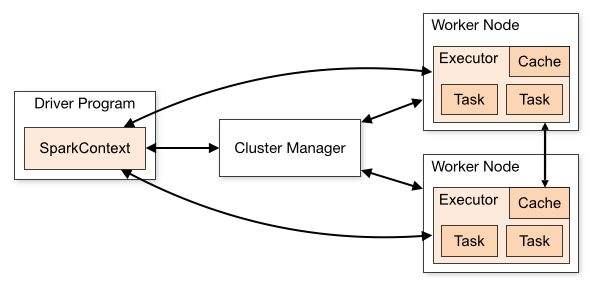
\includegraphics[scale=0.7]{cluster-overview.png}
    \caption{TODO \autocite{Spark2023e}}
\end{figure}

Een van de onderdelen van Hadoop is YARN, een resource manager en job scheduler die instaat voor de verdeling van het werk over de verschillende cluster nodes en dus zorgt voor de schaalbaarheid.
\newline
\begin{figure}
    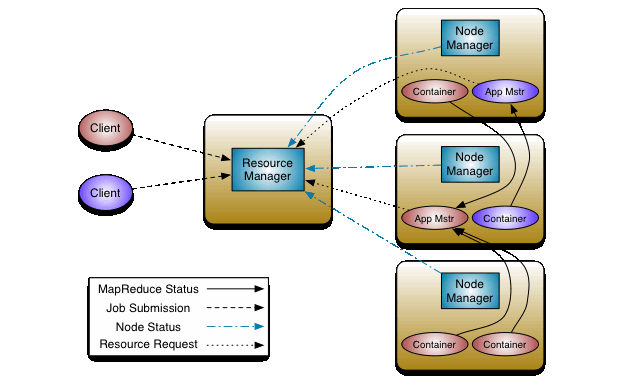
\includegraphics[scale=0.7]{yarn_architecture.png}
    \caption{TODO \autocite{Hadoop2023d}}
\end{figure}

Merk op dat het bij real-world installaties van deze applicaties, het meestal de bedoeling is dat de Big Data oplossingen achterliggend gebruikt worden door eigen applicaties en dat gewone ``gebruikers'' op geen enkele manier rechtstreeks toegang krijgen tot bv. Hadoop of Spark.
\newline
Volgens \autocite{Hadoop2023} wordt in een standaard configuratie de Hadoop cluster eenvoudig beschermd door alle netwerk toegang te beperken. 
Bij de meeste installaties zou dit volstaan als beveiliging, en krijgen enkel de gekende applicaties die er gebruik van maken de netwerk toegang tot de Big Data oplossingen.
\newline
\newline
Dit is niet het geval voor ons, de bedoeling is juist dat de studenten rechtstreeks gebruikmaken van de oplossingen, waarbij één van de doelstellingen van deze bachelorproef is om de verschillende gebruikers (studenten), zowel tijdens de les als tijdens examens volledig afgezonderd te laten werken. Die afzondering geldt zowel op gebied van security als stabiliteit.

\subsection{Security}

\subsubsection{Hadoop Secure mode}
Volgens \textcite{Kiran2022} biedt Hadoop security alle onderdelen van een typische beveiliging: authenticatie, authorisatie, auditing en encryptie van data.
De authenticatie steunt op Kerberos, volgens \textcite{Kerberos2023} een netwerk authenticatie protocol gebaseerd op encryptie en geheime sleutels. Het wordt typisch gebruikt in omgevingen met meerdere partijen die elkaar moeten vertrouwen en waarvoor dus authenticatie vereist is. Er is een implementatie beschikbaar, gemaakt door het MIT en het is beschikbaar zowel als Docker Image als in de typische Linux distributies.
\newline
Volgens \textcite{Hadoop2023} is een zeer goede kennis van Kerberos en DNS vereist om Hadoop services op te zetten in 'secure mode'.
\newline
\newline

\subsubsection{Secure HDFS}
Volgens \textcite{Hadoop2023b} ondersteunt HDFS het gebruik van READ, WRITE en EXECUTE permissies. Daartoe worden alle bestanden en folders geassocieerd met één gebruiker, de eigenaar genoemd, en één groep van gebruikers.
Op die manier kunnen dan permissies toegekend worden aan de eigenaar, aan de groep en aan alle gebruikers. Dit is typisch ook de manier waarop permissies in Linux systemen functioneren.
\newline
Voor gebruikers van Linux komt ook de syntax voor het beheer van de permissies komt bekend voor:
TODO
hdfs dfs –chmod -R go+w <file/dir>


Voorwaarde voor de toepassing van deze permissies is dat de gebruiker is gekend, geauthentificeerd door Kerberos, en dat de groepen waartoe de gebruiker behoort gekend zijn. Voor dit laatste doet HDFS volgens \textcite{Hadoop2023c} een beroep op bijvoorbeeld het Operating Systeem of een LDAP server.


\subsubsection {Spark authenticatie en authorisatie} \autocite{Spark2023c}
Net zoals bij Hadoop zijn security functionaliteiten zoals authenticatie niet actief bij een standaard installatie van Spark. Als er geen afscherming is van de netwerk toegang, moet communicatie tussen de Spark processen afgeschermd worden d.m.v. authenticatie en encryptie, en moet voor de lokale opslag ook encryptie gebruikt worden. De Web User Interface moet beschermd worden door authenticatie, en daarvoor moeten Java servlet filters gebruikt worden, die echter niet door Spark worden aangeboden en dus moeten gebouwd worden op maat van het systeem dat de authenticatie zal doen.
Er zijn voorbeelden te vinden van dit soort filters, meestal gebaseerd op Basic Authentication (zie verder bij nginx). Op volgende blog vind je een voorbeeld van een eigen gebouwde filter die een login pagina toevoegt aan Spark: \textcite{Cacoveanu2019}
\newline
\newline


\subsubsection{Apache Sentry, Apache Ranger, Apache Knox}
Het evolueert allemaal zeer snel in het Hadoop ecosysteem. Volgens \textcite{Chu2020}, een artikel uit 2020 over Hadoop Security, is Apache Sentry de populaire tool voor Authorizatie. Maar kort daarna werd Apache Sentry een verlaten project en is het verhuisd naar de Attic.
\newline
Volgens \textcite{Anand2021} is dit het gevolg van het samengaan van 2 platformen waarbij de keuze is gemaakt om Sentry te vervangen door Ranger. Het artikel bevat een gedetailleerde vergelijking tussen de functionaliteiten van beide oplossingen.
\newline
In https://ysoo23.medium.com/discussion-and-comparison-of-several-hadoop-security-tools-b4532a8c67f9 is er een vergelijking met nog andere tools en daaruit komt Apache Ranger als de beste keuze.


\subsubsection {Kafka}
Volgens \textcite{Maarek2018} ondersteunt Kafka meerdere beveiligingsmechanismes zijnde:
\begin{itemize}
    \item Encryptie van alle data die tussen de Producers, Kafka en de Consumers wordt uitgewisseld. Dit is in ons geval van geen belang, we willen vooral de toegang van de studenten tot elkaars werk afschermen, we gaan er niet van uit dat de gegevens die op het netwerk worden uitgewisseld kwetsbaar zijn gedurende de beperkte periode van een les of examen.
    \item Authenticatie met SSL of SASL: de toegang tot de Kafka cluster wordt enkel toegelaten voor gebruikers die zich kunnen identificeren. Deze identificatie kan met ``SSL'', waarbij de Kafka broker de identititeit van de applicatie verifieerd door middel van SSL certificaten, of met een aantal andere authenticatie mechanismes gaande van PLAINTEXT (eenvoudige gebruikersnaam/paswoord combinatie) tot GSSAPI (Kerberos tickets). Merk op dat ook in deze gevallen SSL wordt gebruikt om op een veilige manier te communiceren.
    \item Authorizatie laat toe om de permissies te definiëren die bepalen of een bepaalde geïdentificeerde gebruiker (applicatie) toegang krijgt tot bepaalde topics om te lezen of the schrijven.
\end{itemize}

Gebruikers afschermen van elkaar in een opstelling van Hadoop en Spark, beiden in clusters wordt snel zeer ingewikkeld. Elk van de oplossingen bestaat uit meerdere processen die met elkaar communiceren en ieder onderdeel moet secure opgezet worden zodat gebruikers niet, bewust of per ongeluk, data van elkaar te zien krijgen. We spreken hier over encryptie voor de opslag, authenticatie en encryptie bij communicatie tussen de verschillende processen, authenticatie voor de gebruiker op Hadoop, authenticatie voor de gebruiker op Spark enz.
De manier van beveiligen is voor elk van deze oplossingen en interne processen op een andere manier, en vraagt om bijkomende softwares zoals LDAP, Kerberos server, enz.

Voor Kafka is de SASL/PLAINTEXT beveiliging zeker voldoende in ons geval en ook relatief eenvoudig op te zetten. Dit gaan we verder dan ook uitproberen.

\subsection{Stabiliteit}
Elk van de Big Data oplossingen, en Kubernetes, ondersteunen mechanismes om applicaties te verdelen over de pods en van elkaar af te schermen, bij bepaalde onderdelen kunnen er limieten gezet worden op CPU en geheugen gebruik. Deze configuraties zijn gekoppeld aan nodes, containers en applicaties. De achterliggende bedoeling is vooral om de eigen gebouwde applicaties te ondersteunen en vlot te laten beroep doen op de Big Data functionaliteiten. De focus van deze mechanismes, dikwijls gebaseerd op een voorkennis van het soort verwerken dat in de cluster zal gebeuren, ligt minder op rechtstreeks gebruik van de oplossingen door gebruikers die applicaties aan het ontwikkelen zijn.
\newline
\newline
In \textcite{Deane2019} wordt hier dieper op ingegaan en wordt gesproken over het ``lawaaierige buurman probleem''. Het legt uit dat hoe meer gebruikers er komen in de cluster, hoe moeilijker het wordt om ervoor te zorgen dat deze gebruikers geen last van elkaar ondervinden. Daartoe passen beheerders allerlei technieken toe zoals YARN resource pools, prioriteiten stellen, specifieke nodes toewijzen aan applicaties, enz. Een aantal van deze technieken zijn ook niet toepasbaar in ons geval want alle ontwikkelaars moeten gelijk behandeld worden, dus prioriteiten zetten is niet haalbaar, en specifiek werk opslitsen op specifieke nodes is ook niet mogelijk tenzij dan door alle ontwikkelaars aparte nodes te geven.
De oplossing die volgens https://blog.cloudera.com/improving-multi-tenancy-with-virtual-private-clusters/ dan typisch gebeurt is opslitsen van de cluster in kleinere clusters. Gezien het hier meestal gaat over dezelfde data van een bedrijf bevat elke cluster dan een duplicaat en hierop gaat het artikel dan verder en stelt een soort tussenmodel voor, waarbij de HDFS data op een gedeelde cluster blijft en de MapReduce en Spark verwerking op aparte clusters gebeurt.
\newline
Aangezien het in ons geval gaat om het gebruik van de cluster door minder ervaren ontwikkelaars, is de kans op ``lawaaierige buren'' groot.


\subsection{Installatie met containertechnologie}
In vorig hoofdstuk kwam de containertechnologie uitgebreid aan bod en gebaseerd op alle informatie die we onderzochten lijkt het gebruik van containers een goede piste om de installatie te vereenvoudigen.
\newline
We zagen ook dat er meerdere mogelijkheden zijn om zo'n installatie op te zetten, zoals Kubernetes, Docker Swarm, Docker Compose, Docker.
\newline
Bij elk van de gebruikte applicaties moeten dus een aanzienlijk aantal nodes opgezet worden voor een basis cluster, gedefinieerd, geconfigureerd en geïnstalleerd.
\newline
De configuratie kan bijvoorbeeld geconfigureerd worden via Kubernetes of Docker Swarm, gedefinieerd in YARN die dan beroep doet op Docker om extra containers te starten. Of volgens \textcite{Spark2023d}, Spark die rechtstreeks kan gebruikmaken van Kubernetes, om Executors op Kubernetes Pods aan te maken en er applicaties op uit te voeren.
\newline
\newline

\subsection{Conclusie}
De eerste vraag die we hier proberen te beantwoorden is of een gedeelde cluster de beste oplossing is voor de oefeningen en het examen van de cursus Big Data. Het alternatief is een aparte omgeving voor elke student.
\newline
De installatie van zowel de gedeelde cluster als de aparte omgeving kan geautomatiseerd worden met voornoemde containertechnologie.
\newline
We zien een aantal mogelijke redenen om te kiezen voor een gedeelde Big Data cluster: reden 1 is gedeelde data, reden 2 is optimaal gebruik van resources en reden 3 is de enkelvoudige installatie t.o.v. een installatie voor elke student.

\subsubsection{Gedeelde data}
Dit is hier niet van toepassing, de data is enerzijds niet van die omvang dat ze niet kan gedupliceerd worden voor elke student en daarnaast is het ook niet de bedoeling dat de studenten dezelfde data kunnen wijzigen.

\subsubsection{Optimaal gebruik van resources}
Hét argument voor optimaal gebruik van resources is dat nodes in een cluster gedeeld worden door alle gebruikers en ter beschikking staan voor het uitvoeren van bewerkingen naargelang de vraag, die niet doorlopend dezelfde is. Op die manier kan aan de afwisselende vraag van de gebruikers worden voldaan door een beperkter aantal nodes dan indien ze vastgelegd zouden zijn per applicatie, en dus gedurende bepaalde ongebruikt zijn.
\newline
In het geval van de studenten is dit niet van toepassing want juist tijdens de oefeningen en het examen wordt er op intensieve manier gebruikt gemaakt van de Big Data cluster en zal een gedeelde cluster voortdurend op piekvermogen moeten draaien.
\newline
Merk op dat het wel waarschijnlijk is dat de installatie van één enkele gedeelde cluster minder resources zal gebruiken dan de aparte omgevingen per student.

\subsubsection{Enkelvoudige installatie}
Het achterliggende idee van gebruik van containertechnologie is dat het eenvoudig is om een container op te starten, te verplaatsen, bijkomende containers te starten, enz. Dit alles gebaseerd op een set Docker images in combinatie met configuratie files.
\newline
Het werk kruipt dus eerder in dit alles opzetten, en is grotendeels onafhankelijk van hoeveel keer het daarna geïnstalleerd moet worden.
Een gedeelde cluster zal complexer zijn om op te zetten door de security en stabiliteitsvereisten.
\newline
Zoals ook aangehaald in het vorige stuk over stabiliteit, zal er altijd het risico blijven dat de studenten niet 100\% afgeschermd zijn van elkaar en van onbetrouwbare applicaties.
\newline
Gebaseerd op het voorgaande lijkt het ons dus beter, en eenvoudiger, is om elke student een eigen omgeving te geven, volledig afgeschermd van de andere, door aparte containers te gebruiken per student.
\newline
De nodige combinaties van containers, nodig voor de oefeningen of het examen, kunnen we opzetten door gebruik te maken van Docker Compose of Kubernetes files die een specifieke combinatie definiëren van de Big Data oplossingen. Voor elke student wordt dan naargelang de les de specifieke omgeving opgestart.
\newline
Merk op dat de Kubernetes of Docker Compose configuratie files die we verder in dit hoofdstuk gaan opbouwen het startpunt zijn voor elk van deze omgevingen, maar niet voldoende. De basis dient aangepast/uitgebreid te worden met specifieke configuraties gerelateerd aan de omgeving, zoals definitie van netwerken en adressen, volumes, enz. Dit dient nog verder uitgewerkt te worden, naargelang de uiteindelijke keuzen van Container Cluster oplossing, om tot een finale oplossing te komen.
\newline
Dit kan uiteindelijk allemaal geautomatiseerd worden maar betekent dat de docent toegang moet hebben tot Kubernetes, Docker Swarm of een VIC UI omgeving om het uit te voeren.
\newline
Een bijkomend voordeel van dit soort aanpak, elke student een eigen omgeving, is dat ze niet alleen kan gebruikt worden om applicaties op de Big Data oplossingen te ontwikkelen, maar ook om studenten de administratie van de Big Data oplossingen zelf op hun eigen geïsoleerde omgeving te leren. Al is dat vandaag niet de focus van de lessen, op hun eigen omgeving kunnen ze Admin zijn zonder impact op anderen.
\newline
\newline


\section{Big data}

Om meer vertrouwd te geraken met de Big Data oplossingen zijn deze eerst allemaal eens lokaal opgezet via Docker Compose configuraties. Zie Appendix [B: Docker compose].
Daarbij is er vertrokken van voorbeelden die beschikbaar zijn op het Internet en voorbeelden uit de Big Data cursusoefeningen.
\newline
\newline
Dit verliep vlot. Pas tijdens het omzetten naar Kubernetes, zie verder, bleek dat het gebruik van Docker en Docker Compose lokaal voor heel wat voordelen zorgt. Bijvoorbeeld dat je eenvoudig een shell kunt openen in om het even welke lokale Docker container en daar commandos kunt uitvoeren die gebruik maken van de geïnstalleerde software in die container. Dit wordt voor de oefeningen gebruikt om bijvoorbeeld Hadoop commandos uit te voeren terwijl er op de lokale machine geen hadoop beschikbaar is. Via 'docker exec' kan de student op de lokale Namenode container aanloggen, er files naar kopiëren en die dan via 'hadoop' commandos naar hdfs in de andere container overbrengen, of Java programma's opstarten.
Eens de lokale omgeving naar de cloud verhuisd zal zijn kan dit niet meer gebruikt worden en moet hiervoor een andere oplossing komen.` Dit gaan we later opnemen en dieper bespreken.'

\section{Security}
We gaan dus niet voor een volledige, alle producten, alle processen, alle communicatie, secure installatie want 1 enkele omgeving voor 1 student zal volledig binnen 1 Pod draaien en in eerste instantie dus ook volledig afgeschermd zijn.
De uitdaging is nu eerder om bepaalde poorten toegankelijk te maken om toe te laten met deze omgeving te werken, maar we willen de toegang tot deze poorten voor elke omgeving wel beperken tot 1 student.

\subsection{Apache Knox}
Zoals eerder al aangehaald is Apache Knox een security oplossing die toe laat een Hadoop cluster af te schermen.
Volgens (https://knox.apache.org/) is het een gateway die de toegang tot de cluster vormt voor alle interacties (REST en HTTP), en die authenticatie doet van de gebruikers. Voor die authenticatie worden de typische protocols ondersteunt zoals LDAP/ActiveDirectory, Kerberos, SAML en OAuth. Dit is ideaal in een onderneming om bestaande gebruikers toe te laten, maar voelt overdreven (overkill) in ons geval van 1 gebruiker per omgeving. Er moest dus naar iets eenvoudigers gezocht worden.

\subsection{Kubernetes services}
Services in Kubernetes zijn een manier om toegang te verlenen tot de netwerk applicaties die in één of meerdere Pods in de cluster draaien. Aangezien deze applicaties op elk moment van Pod kunnen wijzigen of in meerdere Pods opgestart worden, is er een mechanisme nodig die dit opvangt en zorgt dat de applicaties toegankelijk blijven voor de buitenwereld. Dit zijn de Kubernetes Services.
\autocite{Kubernetes2023b}

Er zijn meerdere types services maar voor onze oplossing is het Ingress type van belang omdat het gewoon een HTTP(S) ingangspunt is in combinatie met regels voor routing. Achterliggend is 1 van de implementaties de Ingress-Nginx controller. Dit is een integratie van Nginx uitgebreid met Kubernetes integratie mechanismes voor o.a. herstarten/herladen bij configuratie wijzigingen. Bij onze opzet zijn er geen wijzigingen eens de omgeving is opgestart, dus heb werd er een test opgezet met een gewone Nginx die dan deel uitmaakt van de Kubernetes Pod.
\autocite{Kubernetes2023d}


\subsection{Nginx}
Nginx (https://www.nginx.com/) is een web server die dikwijls als ingangspunt van een web site gebruikt wordt (Reverse proxy TODO \autocite{Wikipedia2023d}) en die zorgt dat de achterliggende structuur afgeschermd is voor de buitenwereld. Daarnaast kan het zorgen voor Load Balancing TODO \autocite{Wikipedia2023c} en beveiliging (HTTP Basic Authentication, SSL/TLS offloading).
\newline
\newline


\subsubsection{HTTP Basic Authentication}
TODO \autocite{Wikipedia2023b}
Basic Authentication is een optioneel onderdeel van een HTTP(S) transactie waarbij aan de initiërende partij, typisch de webbrowser, gevraagd wordt een gebruikersnaam en paswoord te verstrekken. Het is de eenvoudigste techniek voor het afdwingen van toegangscontroles tot web resources, omdat hiervoor geen cookies, sessie-ID's of inlogpagina's nodig zijn.
Omdat de inloggegevens in de header van elk HTTP(S)-verzoek moeten worden verzonden, moet de webbrowser ze gedurende een redelijke tijd in de cache opslaan om te voorkomen dat de gebruiker voortdurend om zijn gebruikersnaam en wachtwoord wordt gevraagd.
Merk op dat de inloggegevens die verstuurd worden (gebruikersnaam en paswoord) niet beschermd zijn, ze zijn gecodeerd met base64 encoding maar dit biedt geen enkele bescherming. Daarom wordt Basic Authentication meestal gebruikt in combinatie met HTTPS om vertrouwelijkheid te bieden. Aangezien het in onze oplossing over tijdelijke omgevingen gaat is het gevaar dat bij HTTP de inloggegevens onderschept worden minimaal en kan dit dus ook voor niet-HTTPS gebruikt worden.
\newline
\newline
Basic Authentication lijkt me voldoende, per omgeving moeten dan de inloggegevens voor 1 gebruiker, de student, opgezet worden. Nginx ondersteunt meerdere mechanismen voor authenticatie waaronder een eenvoudig paswoord bestand. Deze is in het formaat
\newline
\newline
\begin{lstlisting}
user1:$apr1$/woC1jnP$KAh0SsVn5qeSMjTtn0E9Q0
user2:$apr1$QdR8fNLT$vbCEEzDj7LyqCMyNpSoBh/
user3:$apr1$Mr5A0e.U$0j39Hp5FfxRkneklXaMrr/ 
\end{lstlisting}


en wordt gegenereerd door Linux tools zoals htpasswd (deel van apache2-utils en httpd-tools), waarbij het paswoord van een gebruiker met MD5 wordt geëncrypteerd. In ons geval zou dit bestand dus de unieke student gebruiker bevatten, met verschillend paswoord per omgeving.
Optioneel kan overal een extra account voor de lesgever, met identiek paswoord voor alle omgevingen, toegevoegd worden.
\newline
\newline
Als eerste onderzoek voor dit security onderdeel is er, om de configuratie van de Basic Authenticatie te bouwen, een beperkte Kubernetes yaml file gemaakt met alleen maar nginx, deze start en stopt snel tijdens het testen, maar liet al direct toe om Kubernetes Services, Port mapping en Configmap te gebruiken. Dit was ook de eerste keer dat Kubernetes werd gebruikt en dus lokaal moest geïnstalleerd worden.
\newline
\newline
\subsubsection{Configmaps} 
\autocite{Kubernetes2023}
\newline
Een ConfigMap wordt gebruikt om niet-beveiligde configuratie gegevens te beheren in sleutel-waarde formaat, en ter beschikking te stellen van de Pods en Containers, als omgevingsvariabele of als (configuratie) bestand via een volume.
Een ConfigMap bevat typisch de configuratie die is losgekoppeld van het Docker image om op die manier images meer generiek inzetbaar te maken.\textcite{Kubernetes2023}


Initieel waren er hier problemen met het configureren van de volumes omdat Kubernetes volumes op een andere manier werken dan de volumes van Docker Compose, waar er eenvoudig verwezen kan worden naar lokale folders op de machine waar de container draait, terwijl bij Kubernetes alles in de Configmap gestopt wordt om op die manier van Pod te kunnen switchen of uitbreiden, en de configuratie (files) mee moet kunnen naar alle pods.
\newline
\newline
In de ConfigMap werd de nginx.conf file gestopt en de paswoord file voor Basic Authentication.
Uiteindelijk met volgende configuratie kwam de popup voor Basic Authentication te voorschijn.
\newpage
\begin{lstlisting}
user  nginx;
worker_processes  1;

error_log  /var/log/nginx/error.log warn;
pid        /var/run/nginx.pid;

events {
    worker_connections  1024;
}
http {
    include       /etc/nginx/mime.types;
    
    default_type  application/octet-stream;
    
    log_format  main  '$remote_addr - $remote_user [$time_local] "$request" '
    '$status $body_bytes_sent "$http_referer" '
    '"$http_user_agent" "$http_x_forwarded_for"';
    
    access_log  /var/log/nginx/access.log  main;
    
    sendfile        on;
    
    keepalive_timeout  65;
    
    server {
        listen 443 ssl;
        listen [::]:443 ssl;
        
        server_name         www.hadoop.local;
        ssl_certificate     /etc/nginx/ssl/tls.crt;
        ssl_certificate_key /etc/nginx/ssl/tls.key;
        ssl_protocols       TLSv1 TLSv1.1 TLSv1.2;
        ssl_ciphers         HIGH:!aNULL:!MD5;
        
        proxy_set_header Host $host;
        proxy_set_header X-Forwarded-For $proxy_add_x_forwarded_for;
        
        proxy_cache_revalidate on;
        proxy_cache_use_stale error timeout http_500 http_502 http_503 http_504;
        proxy_cache_background_update on;
        proxy_cache_lock on;
        
        resolver kube-dns.kube-system.svc.cluster.local valid=5s;
        
        auth_basic "Access restricted";
        auth_basic_user_file /etc/nginx/password.conf;
        
        location / {
            root /usr/share/nginx/html;
            index index.html index.htm;
        }
    }
}
\end{lstlisting}

[TODO] - Eigen Docker image voor nginx docker + config via ENV
Hier is nog een idee om verder te automatiseren door aan de Nginx Docker container de gebruikersnaam en paswoord te geven en die gaat dan intern htpasswd gebruiken om de Auth file te genereren. Nog verder uit te werken ?
https://github.com/dtan4/nginx-basic-auth-proxy
\newline
\newline
\begin{lstlisting}
version: '2'
services:
web:
image: tutum/hello-world:latest
nginx:
image: quay.io/dtan4/nginx-basic-auth-proxy:latest
ports:
- 8080:80
- 8090:8090
environment:
- BASIC_AUTH_USERNAME=username
- BASIC_AUTH_PASSWORD=password
- PROXY_PASS=http://web/
- PROXY-SERVERNAME=hadoop.student1.hogent.be

\end{lstlisting}

\section{Hadoop}
Daarna werd Hadoop toegevoegd en de configuratie voor nginx om als Reverse Proxy gebruikt te worden voor Hadoop. Hierbij is vertrokken van de Docker Compose file die was opgebouwd en getest in vorige stappen, en heb die toegevoegd aan de Kubernetes file maar bij het opstarten waren er een aantal problemen. De namenode was niet bereikbaar voor de datanode, resourcemanager en historyserver.
In een Docker compose file worden alle containers verbonden via 1 of meerdere virtuele netwerken, en zorgt Docker ervoor dat de containers naar elkaar kunnen verwijzen door middel van de containernaam. Dit is niet het geval bij Kubernetes (of vSphere), waar de naam van de Pod, waarop de container draait, moet worden gebruikt. Aangezien in onze oplossing alle containers voor 1 student op dezelfde Pod draaien kunnen we ook 'localhost' gebruiken.\newline
In de configuratie voor Kubernetes moest dus bij elke container de verwijzing naar andere containers (hostnamen) vervangen worden door 'localhost'.
\newline
\newline
Om de configuratie van Hadoop aan te passen zijn er 2 manieren, ofwel gebruikmakende van environment variabelen gedefinieerd rechtstreeks op de container ofwel met environment variabelen gedefinieerd in een aparte ConfigMap. Typisch worden beiden gebruikt, in de ConfigMap stoppen we variabelen die voor alles containers gelijk zijn, op de container de variabelen die verschillend zijn per container. Een voorbeeld van de laatste soort is SERVICE\_PRECONDITION die een manier is om de bepalen op welke andere containers moet gewacht worden. Dit is een mechanisme van Apache, waarbij een specifieke applicatie wacht met opstarten tot het contact krijgt met die andere applicatie.
\newline
\newline
Na deze aanpassingen leek het nog niet voldoende om alles werkend te krijgen maar uiteindelijk bleek het te liggen aan de ConfigMap die ook nog elementen van nginx bevatte.
\newline
\newline
Eens Hadoop werkende in Kubernetes, werd de reverse proxy configuratie van nginx aangepakt. Eerst door een Hadoop context toe te voegen aan de URL, bv http://localhost/hadoop, en die dan via de nginx proxy\_pass door te sturen naar Hadoop.
\newline
\newline
\begin{lstlisting}
location / {
    proxy_set_header Host $http_host;
    proxy_redirect off;
    # rewrite ^/hadoop/(.*)$ /$1 break;
    proxy_pass http://localhost:9870/;
}

\end{lstlisting}

Daarbij trad volgend probleem op:
\newline
\newline
- Browser vraagt http://localhost/hadoop
- Browser krijgt HTML terug van Hadoop, via nginx
- HTML bevat verwijzingen naar /static/bootstrap.css
\newline
\newline
Een mogelijke oplossing hiervoor is ofwel nginx de HTML te laten aanpassen (filteren) en regels te definiëren die overal '/hadoop' toevoegen aan links van images, css, enz. Hierbij is er een kans dat we niet alle gevallen vinden en toevoegen aan de filter.
Een andere oplossing is om een apart DNS adres (servernaam) te gebruiken voor Hadoop, nginx kan dan op basis van de servernaam de requests doorsturen naar Hadoop. Hiervoor moest lokaal de hosts file van Windows 
\newline
(C:/Windows/System32/drivers/etc) gewijzigd worden en het volgende toegevoegd:
127.0.0.1 www.hadoop.local
\newline
\newline
De reverse proxy configuratie moest ook aangepast worden omdat het niet langer op url (location /hadoop) werkt maar op servernaam.
\newline
\newline
\begin{lstlisting}
server {
    listen 80;
    listen [::]:80;
    server_name localhost;
}

\end{lstlisting}

Bij surfen in de browser naar http://www.hadoop.local, kwam er nu eerst de user/paswoord popup en pas na invullen van de correcte gegevens kwam de WebUI van Hadoop.

\section{HTTPS/SSL}

Om de installatie veiliger te maken is er beslist om HTTPS op te zetten. Het is voldoende om dit op nginx te configureren want dat is de enige server en communicatie die van buitenaf zichtbaar is en dus mogelijk kan bespioneerd worden. Er zijn nog een aantal voordelen dat dit enkel op de nginx server moet gebeuren:
\newline
\newline
- Performantie: SSL maakt zwaar gebruik van de CPU en op deze manier worden de andere containers hiermee niet belast.
- Certificaat beheer: installatie en onderhoud van de certificaten moet maar op 1 plaats gebeuren
- SSL software patching: indien kwetsbaarheden ontdekt worden in de SSL software moet de installatie van security patches enkel op de nginx gebeuren, eenvoudig door naar een nieuw image te verwijzen.
\newline
\newline
Het opzetten van SLL op een aparte server, nginx in dit geval noemt men 'SSL offloading'.

\subsection{Certificaat}

Om SSL op te zetten bij nginx is een certificaat nodig. Voor de lokale testen werd er een certificaat gegenereerd gebruikt makende van openssl. Aangezien dit niet standaard al op Windows geïnstalleerd is, is er een tijdelijke Docker image gebruikt: alpine/openssl.
\newline
\newline
Met volgende commando kon werd een certificaat aangemaakt dat vanuit de Docker container bewaard werd op de laptop.
\newline
\newline

docker run -ti --rm -v \$(pwd):/apps -w /apps alpine/openssl <openssl\_command>

\begin{lstlisting}
server {
    listen              443 ssl;
    server_name         www.hadoop.local;
    ssl_certificate     /etc/nginx/ssl/tls.crt;
    ssl_certificate_key /etc/nginx/ssl/tls.key;
    
    location / {
        proxy_pass ...
    }
}
\end{lstlisting}

\section{Spark}

De volgende stap was een Kubernetes yaml bestand voor de combinatie Nginx, Hadoop en Spark. Dit verliep vlot, dezelfde problemen als bij Hadoop, vooral docker container namen die omgezet moesten worden naar localhost, enz die we intussen al snel herkenden.
\newline
\newline
Docker Compose biedt een functionaliteit die in Kubernetes niet bestaat, namelijk 'depends\_on'. Deze laat toe om de afhankelijkheid van containers te definiëren zodat containers niet starten voordat andere nodige containers zijn gestart. Dit wordt gebruikt bij Spark worker die (depends\_on) Spark master nodig heeft.
Bij Hadoop wordt dit opgelost door een eigen aanpak, de SERVICE\_PRECONDITION (zie eerder vermeld bij Hadoop).
\newline
\newline
Spark heeft daar geen oplossing voor maar uiteindelijk bleek dat de Spark processen hier geen hinder van ondervonden en dus het gebrek aan de 'depends\_on' geen probleem vormt.
\newline
\newline
Net zoals bij Hadoop werd dan bij nginx een servernaam geconfigureerd voor de reverse proxy, en de naam lokaal toegevoegd aan de hosts file:
127.0.0.1 www.spark.local
\newline
\newline
Wie daarna in de browser naar https://www.spark.local ging, kreeg eerst de user/paswoord popup en na invullen van de correcte gegevens zag die de WebUI van Spark.

\section{Kafka}

Als laatste werden Kafka en Zookeeper opgezet in een Kubernetes configuratie. Ook hier weer zat de complexiteit in het vervangen van de juiste servernaam configuraties door localhost en openzetten van de juiste poorten.
Dit is nog een verschil met Docker Compose, namelijk de containers in een Compose bestand kunnen vrij met elkaar communiceren over alle poorten, de poorten die in een Compose gedefinieerd worden zijn de poorten die van buitenaf toegankelijk moeten zijn. Bij Kubernetes moeten alle nodige poorten ook op elke container opengezet worden via configuratie.
\newline
\newline
Als voorbeeld was er vertrokken van een configuratie met 3 Kafka brokers maar dit werd te zwaar voor de laptop in combinatie met alles van Kubernetes. Bij wijzigen van configuratie en herstarten van containers ging de Disk usage regelmatig naar 100\% en moest de laptop herstart worden.
Dus is er verdergegaan met een opzet met 1 Kafka broker en 1 Zookeeper.
\newline
\newline
Kafka ondersteunt meerder beveiligingsmechanismes waaronder SASL/PLAIN, een eenvoudige authenticatie gebaseerd op gebruikersnamen en paswoorden in een bestand.
\newline
\newline
Dit kan opgezet worden in een ConfigMap, dit is nog niet gebeurd door tijdsgebrek. (Voorlopig)
\newline
\newline

\begin{figure}
    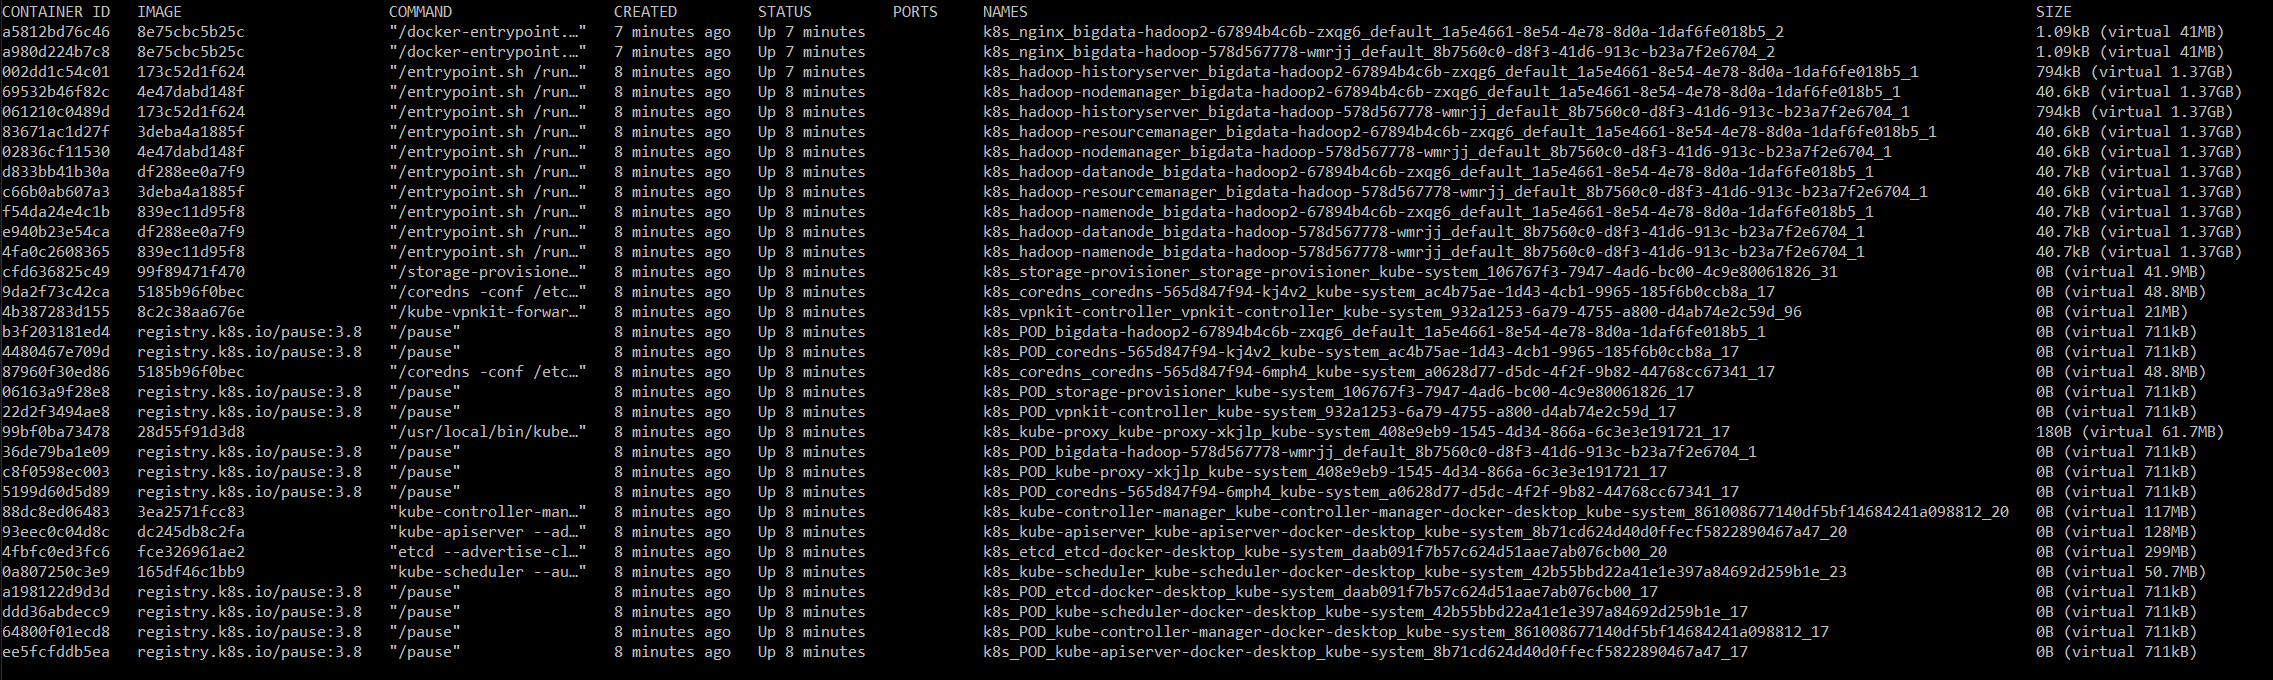
\includegraphics[scale=0.4]{Hadoop 2 pods resource usage size.png}
    \caption{TODO}
\end{figure}

\begin{figure}
    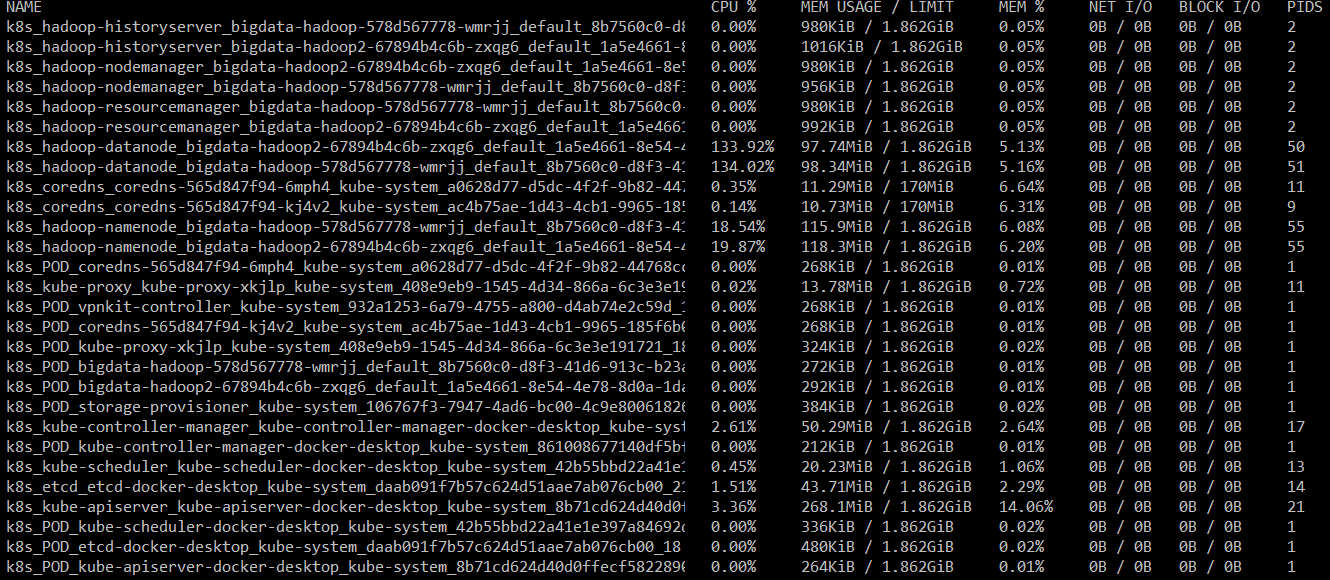
\includegraphics[scale=0.4]{Hadoop 2 pods resource usage.png}
    \caption{TODO}
\end{figure}

\begin{figure}
    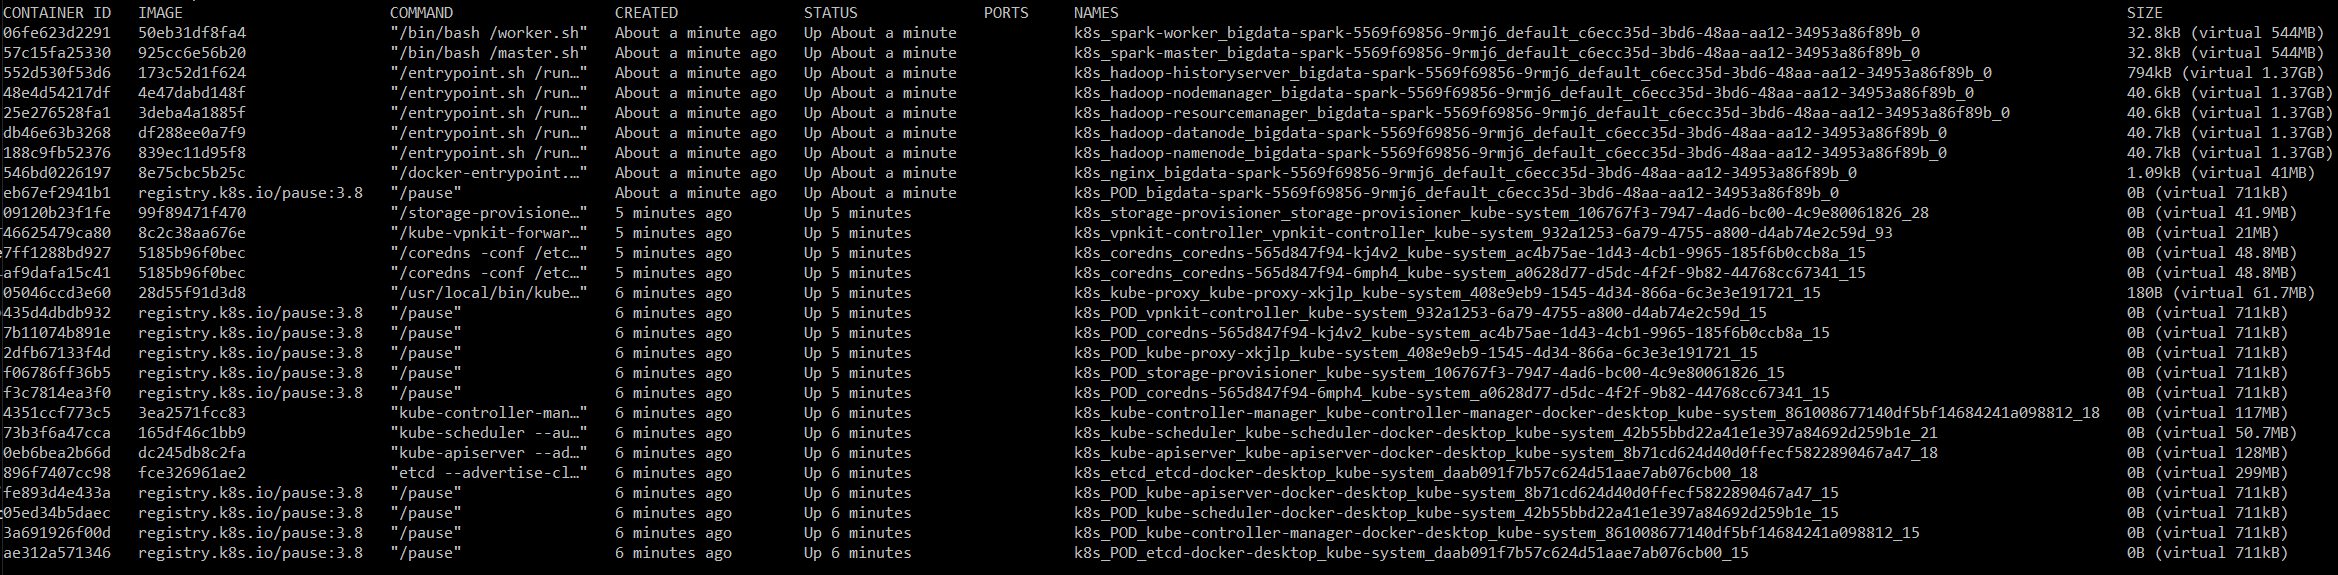
\includegraphics[scale=0.4]{Hadoop and Spark resource usage size.png}
    \caption{TODO}
\end{figure}

\begin{figure}
    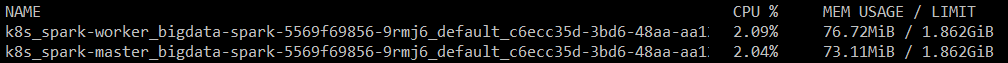
\includegraphics[scale=0.4]{Hadoop and Spark resource usage.png}
    \caption{TODO}
\end{figure}

\begin{figure}
    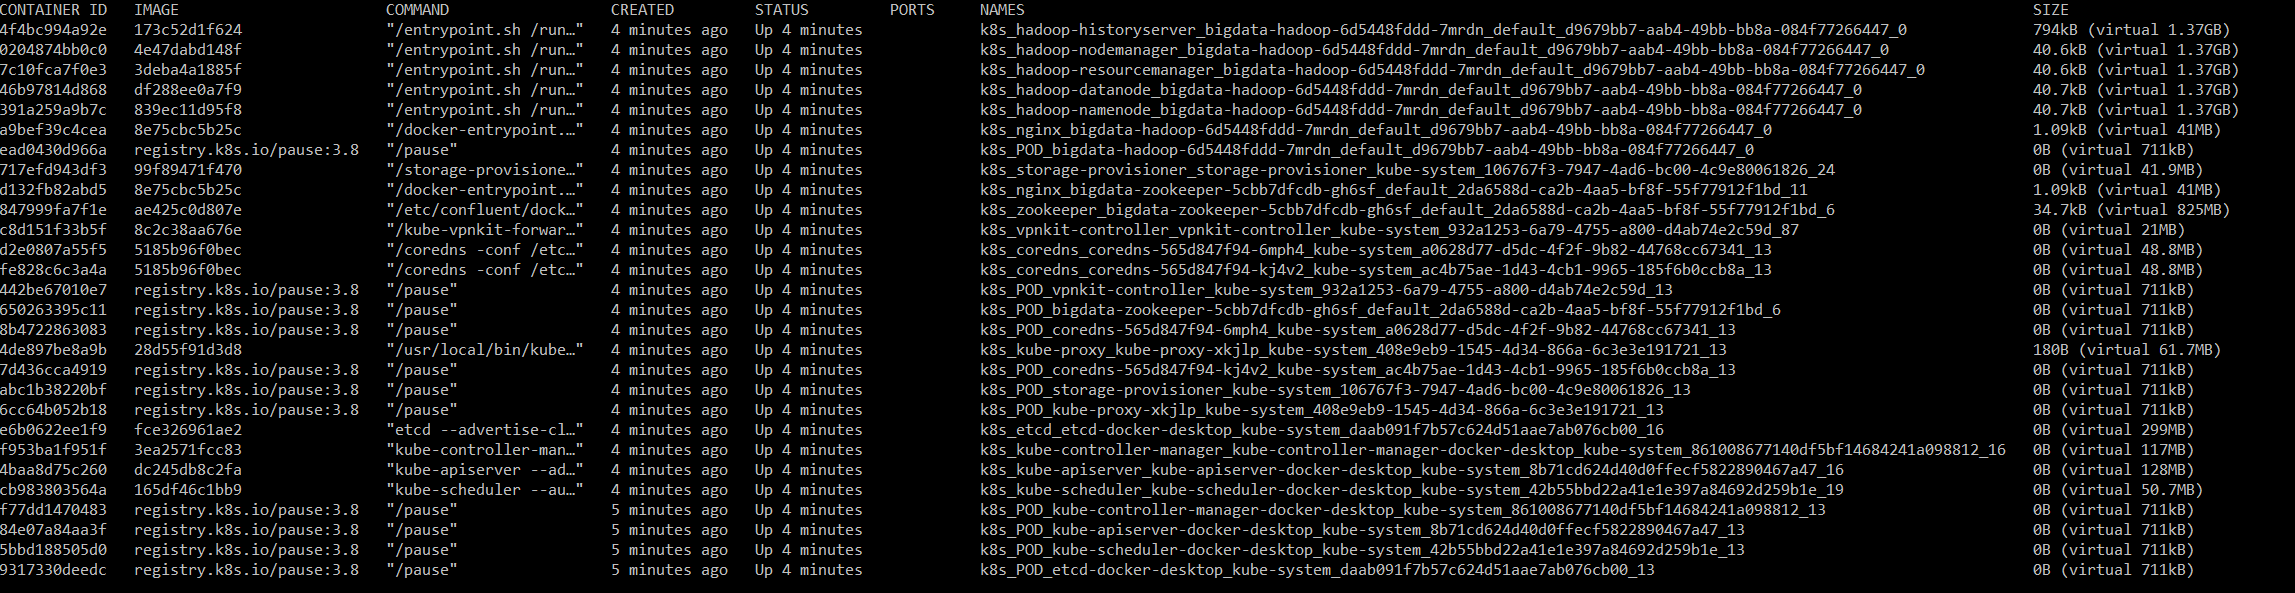
\includegraphics[scale=0.4]{Hadoop resource usage size.png}
    \caption{TODO}
\end{figure}

\begin{figure}
    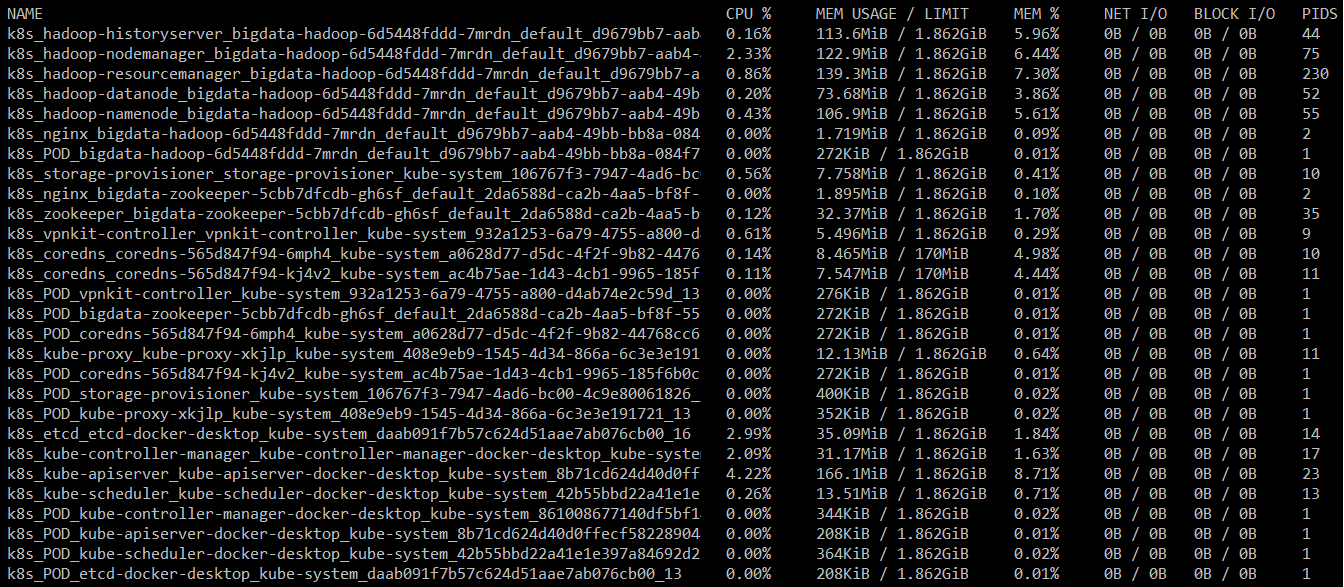
\includegraphics[scale=0.4]{Hadoop resource usage.png}
    \caption{TODO}
\end{figure}

\begin{figure}
    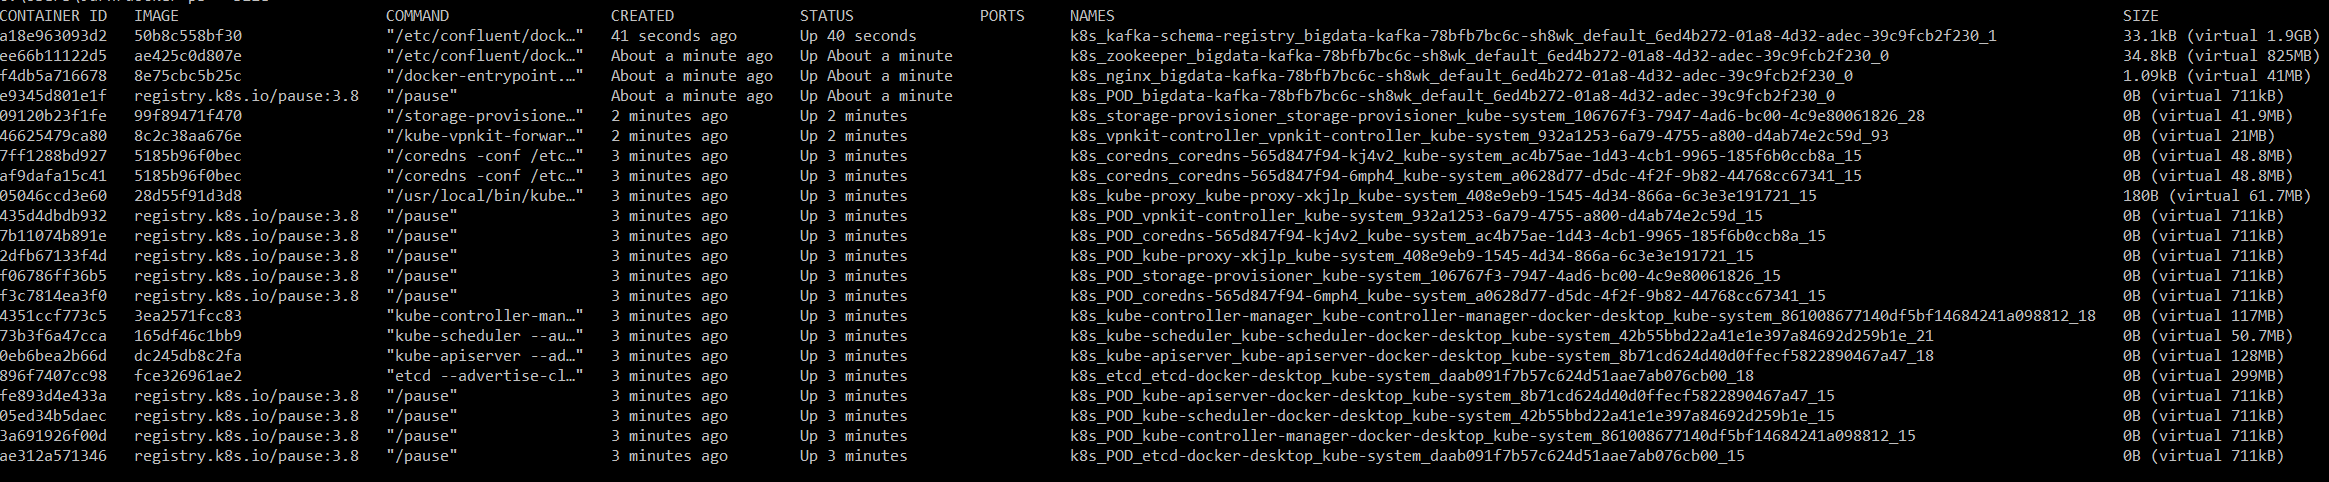
\includegraphics[scale=0.4]{Kafka resource usage size.png}
    \caption{TODO}
\end{figure}

\begin{figure}
    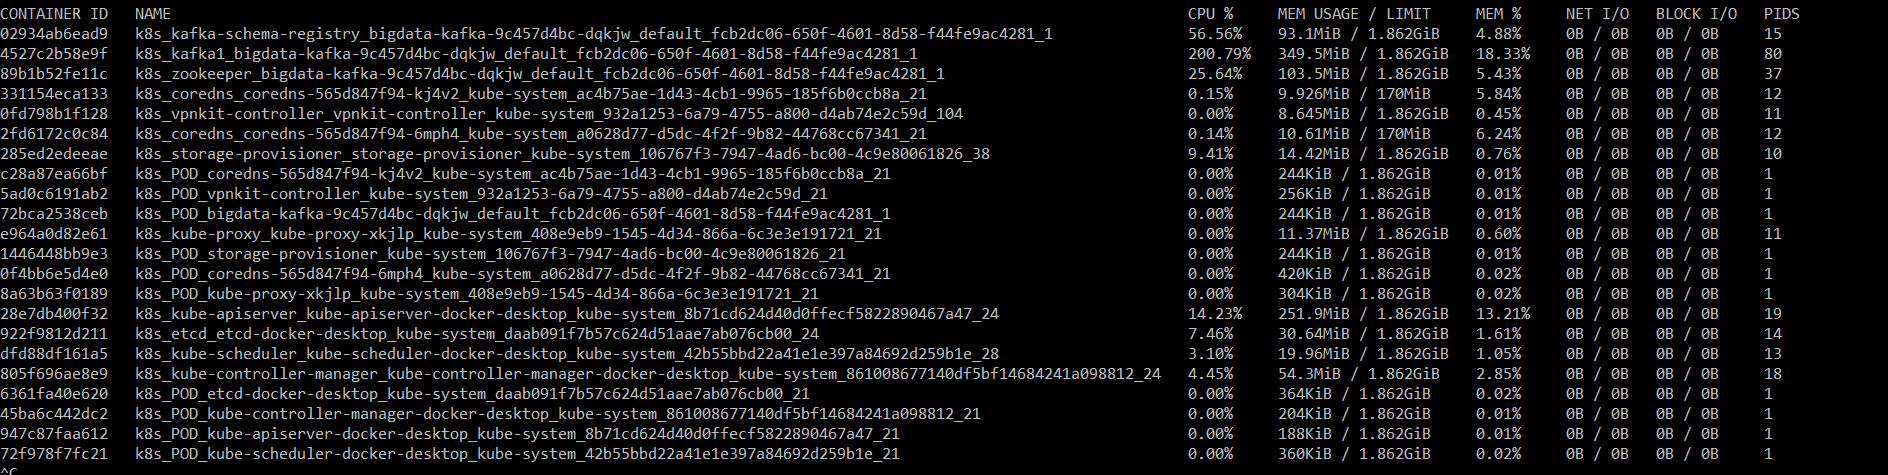
\includegraphics[scale=0.4]{Kafka resource usage.png}
    \caption{TODO}
\end{figure}
